%\chapter{Tracing}
\chapter{トレース}
\label{chap:tracing}

%One of the lesser known and absolutely under-used features of Erlang and the BEAM virtual machine is just about how much tracing you can do on there.
ErlangとBEAM VMの機能で、およそどれぐらいのことをトレースできるかはあまり知られておらず、また全然使われていません。

%Forget your debuggers, their use is too limited.\footnote{One common issue with debuggers that let you insert break points and step through a program is that they are incompatible with many Erlang programs: put a break point in one process and the ones around keep going. In practice, this turns debugging into a very limited activity because as soon as a process needs to interact with the one you're debugging, its calls start timing out and crashing, possibly taking down the entire node with it. Tracing, on the other hand, doesn't interfere with program execution, but still gives you all the data you need.} Tracing makes sense in Erlang at all steps of your system's life cycle, whether it's for development or for diagnosing a running production system.
使えるところが限られているので、デバッガのことは忘れてください\footnote{デバッガでブレークポイントを追加してステップ実行する時の代表的な問題は、多くのErlangプログラムとうまくやりとりができないことです。あるプロセスがブレークポイントで止まっても、その他のプロセスは動作し続けます。そのため、プロセスがデバッグ対象のプロセスとやりとりが必要なときにはすぐに、プロセス呼び出しがタイムアウトしてクラッシュし、おそらくノード全体を落としてしまいます。ですから、デバックは非常に限定的なものとなります。一方でトレースはプログラムの実行を邪魔することは無く、また必要なデータをすべて取得することができます。}。Erlangでは、トレースは開発中あるいは稼働中の本番システムの診断など、システムのライフサイクルのどこでも便利です。

%There are a few options available to trace Erlang programs:
トレースを行ういくつかのErlangプログラムがあります。


\begin{itemize}
%	\item \module{sys}\footnote{\href{http://www.erlang.org/doc/man/sys.html}{http://www.erlang.org/doc/man/sys.html}} comes standard with OTP and allows the user to set custom tracing functions, log all kinds of events, and so on. It's generally complete and fine to use for development. It suffers a bit in production because it doesn't redirect IO to remote shells, and doesn't have rate-limiting capabilities for trace messages. It is still recommended to read the documentation for the module.
	\item \module{sys}\footnote{\href{http://www.erlang.org/doc/man/sys.html}{http://www.erlang.org/doc/man/sys.html}} はOTPに標準で付属されており、利用者はトレース機能のカスタマイズや、あらゆる種類のイベントのロギングなどができます。多くの場合、開発用として完全かつ最適です。一方で、IOをリモートシェルにリダイレクトしないですし、メッセージのトレースのレート制限機能を持たないため、本番環境にはあまり向きません。このモジュールのドキュメントを読むことをお勧めします。

%	\item \otpapp{dbg}\footnote{\href{http://www.erlang.org/doc/man/dbg.html}{http://www.erlang.org/doc/man/dbg.html}} also comes standard with Erlang/OTP. Its interface is a bit clunky in terms of usability, but it's entirely good enough to do what you need. The problem with it is that you \emph{have to know what you're doing}, because \otpapp{dbg} can log absolutely everything on the node and kill one in under two seconds.
\item \otpapp{dbg}\footnote{\href{http://www.erlang.org/doc/man/dbg.html}{http://www.erlang.org/doc/man/dbg.html}}も Erlang/OTPに標準で付属しています。使い勝手の面ではインターフェースは少しイケてませんが、必要なことをやるには十分です。問題点としては、\emph{何をやっているのか知らないといけない}ということです。なぜなら \otpapp{dbg} はノードのすべてをロギングすることや、2秒もかからずにノードを落とすこともできるからです。

%	\item \emph{tracing BIFs} are available as part of the \module{erlang} module. They're mostly the raw blocks used by all the applications mentioned in this list, but their lower level of abstraction makes them rather difficult to use.
	\item \emph{トレースBIF}は \module{erlang}モジュールの一部として提供されています。このリストの全てのアプリケーションで使われているローレベルの部品ですが、抽象化が低いため、利用するのは困難です。

%\item \otpapp{redbug}\footnote{\href{https://github.com/massemanet/eper/blob/master/doc/redbug.txt}{https://github.com/massemanet/eper/blob/master/doc/redbug.txt}} is a production-safe tracing library, part of the \otpapp{eper}\footnote{\href{https://github.com/massemanet/eper}{https://github.com/massemanet/eper}} suite. It has an internal rate-limiter, and a nice usable interface. To use it, you must however be willing to add in all of \otpapp{eper}'s dependencies. The toolkit is fairly comprehensive and can be a very interesting install.
\item \otpapp{redbug}\footnote{\href{https://github.com/massemanet/eper/blob/master/doc/redbug.txt}{https://github.com/massemanet/eper/blob/master/doc/redbug.txt}} は \otpapp{eper}\footnote{\href{https://github.com/massemanet/eper}{https://github.com/massemanet/eper}} スイートの一部で、本番環境環境でも安全に使えるトレースライブラリです。内部にレート制限機能を持ち、使いやすい素敵なインターフェースを持っていますが、利用するには\otpapp{eper}が依存するもの全てを追加する必要があります。ツールキットは包括的で、またインストールは非常に面白いです。

%\item \module{recon\_trace}\footnote{\href{http://ferd.github.io/recon/recon\_trace.html}{http://ferd.github.io/recon/recon\_trace.html}} is \otpapp{recon}'s take on tracing. The objective was to allow the same levels of safety as with \otpapp{redbug}, but without the dependencies. The interface is different, and the rate-limiting options aren't entirely identical. It can also only trace function calls, and not messages.\footnote{Messages may be supported in future iterations of the library. In practice, the author hasn't found the need when using OTP, given behaviours and matching on specific arguments allows the user to get something roughly equivalent.}
\item \module{recon\_trace}\footnote{\href{http://ferd.github.io/recon/recon\_trace.html}{http://ferd.github.io/recon/recon\_trace.html}}は\otpapp{recon}によるトレースです。\otpapp{redbug}と同程度の安全性を目的としていましたが、依存関係はありません。インターフェースは異なり、またレート制限のオプションも完全に同じではありません。関数呼び出しもトレースすることができますが、メッセージのトレースはできません\footnote{メッセージのトレース機能は将来のバージョンでサポートされるかもしれません。ライブラリの著者は OTP を使っている時には必要性を感じておらず、またビヘイビアと特定の引数へのマッチングにより、ユーザはおよそ同じことを実現できます}。
\end{itemize}

この章では \module{recon\_trace} によるトレースにフォーカスしていきますが、使われている用語やコンセプトの多くは、Erlang の他のトレースツールにも活用できます。

%\section{Tracing Principles}
\section{トレースの原則}
\label{sec:tracing-princples}

%The Erlang Trace BIFs allow to trace any Erlang code at all\footnote{In cases where processes contain sensitive information, data can be forced to be kept private by calling \expression{process\_flag(sensitive, true)}}. They work in two parts: \emph{pid specifications}, and \emph{trace patterns}.
ErlangのトレースBIFは全てのErlangコードをトレースすることを可能にします\footnote{プロセスに機密情報が含まれている場合、\expression{process\_flag(sensitive, true)}を呼ぶことで、データを非公開にすることを強制できます}。BIFは\emph{pid指定}と\emph{トレースパターン}に分かれています。

%Pid specifications lets the user decide which processes to target. They can be specific pids, \expression{all} pids, \expression{existing} pids, or \expression{new} pids (those not spawned at the time of the function call).
pid指定により、ユーザはどのプロセスをターゲットにするかを決めることができます。pidは、特定のpid, \expression{全ての}pid, \expression{既存の}pid, あるいは \expression{new} pid(関数呼び出しの時点ではまだ生成されていないプロセス)で指定できます。

%The trace patterns represent functions. Functions can be specified in two parts: specifying the modules, functions, and arity, and then with Erlang match specifications\footnote{\href{http://www.erlang.org/doc/apps/erts/match\_spec.html}{http://www.erlang.org/doc/apps/erts/match\_spec.html}} to add constraints to arguments.
トレースパターンは関数の代わりになります。関数の指定は2つに分かれており、MFA(モジュール、関数、アリティ)と Erlang のマッチの仕様で引数に制約を加えています\footnote{\href{http://www.erlang.org/doc/apps/erts/match\_spec.html}{http://www.erlang.org/doc/apps/erts/match\_spec.html}}

%What defines whether a specific function call gets traced or not is the intersection of both, as seen in Figure~\ref{fig:tracing-venn}.
特定の関数呼び出しがトレースされるかどうかを定義している箇所は、~\ref{fig:tracing-venn}にあるように、両者の共通部分です。

\begin{figure}[H]
  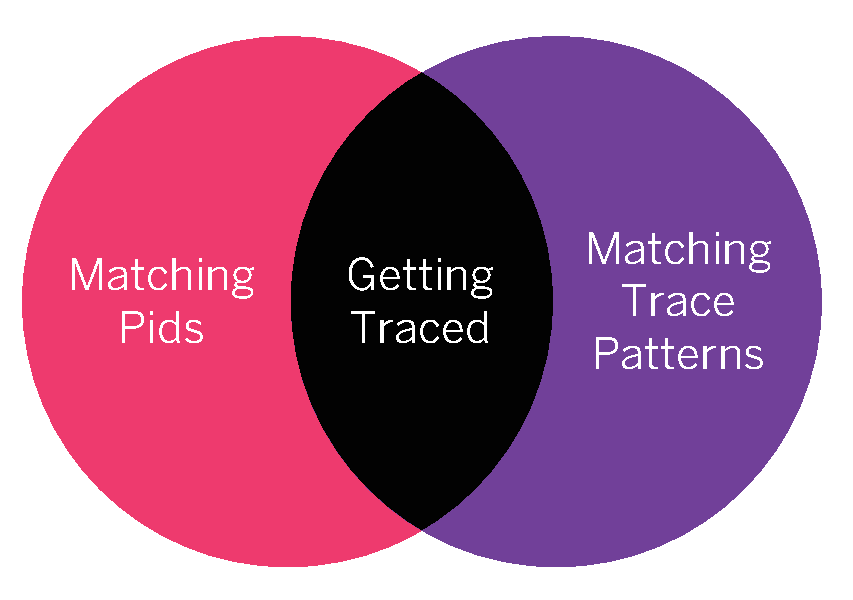
\includegraphics[max height=7cm]{tracing-venn.pdf}%
  \centering%
%  \caption{What gets traced is the result of the intersection between the matching pids and the matching trace patterns}%
  \caption{トレースされるのは、pid指定とトレースパターンの交差した箇所です}%
   \label{fig:tracing-venn}
\end{figure}

%If either the pid specification excludes a process or a trace pattern excludes a given call, no trace will be received.
pid指定がプロセスを除外、あるいはトレースパターンが指定の呼び出しを除外した場合、トレースは受信されません。

%Tools like \otpapp{dbg} (and trace BIFs) force you to work with this Venn diagram in mind. You specify sets of matching pids and sets of trace patterns independently, and whatever happens to be at the intersection of both sets gets to be displayed.
\otpapp{dbg}(およびトレースBIF)のようなツールは、このベン図を念頭に置いて作業することを前提としています。pid指定およびトレースパターンを別々に指定し、その結果が何であろうとも、両者の共通部分が表示されることになります。

%Tools like \otpapp{redbug} and \module{recon\_trace}, on the other hand, abstract this away.
一方で \otpapp{redbug}や\module{recon\_trace}のようなツールでは、これらを抽象化しています。

%\section{Tracing with Recon}
\section{Recon によるトレース}

%Recon, by default, will match all processes. This will often be good enough for a lot of debugging cases. The interesting part you'll want to play with most of the time is specification of trace patterns. Recon support a few basic ways to declare them. 
デフォルトでは Recon は全てのプロセスにマッチしますが、デバッグ時のほとんどのケースはこれで問題ありません。多くの場合、あなたがいじくりたいと思う面白い部分は、トレースするパターンの指定です。Recon ではいくつかの方法をサポートしています。

%The most basic form is \expression{\{Mod, Fun, Arity\}}, where \var{Mod} is a literal module, \var{Fun} is a function name, and \var{Arity} is the number of arguments of the function to trace. Any of these may also be replaced by wildcards (\expression{'\_'}). Recon will forbid forms that match too widely on everything (such as \expression{\{'\_','\_','\_'\}}), as they could be plain dangerous to run in production.
最も基本的な指定方法は \expression{\{Mod, Fun, Arity\}}で、\var {Mod} はモジュール名、\var{Fun}は関数名、\var{Arity} はアリティつまりトレース対象の関数の引数の数です。いずれもワイルドカードの(\expression{'\_'})で置き換えることができます。本番環境での実行は明らかに危険なため、Recon は(\expression{\{'\_','\_','\_'\}}のように)あまりにも広範囲あるいは全てにマッチするような指定は禁止しています。

%A fancier form will be to replace the arity by a function to match on lists of arguments. The function is limited to those usable by match specifications similar to what is available in ETS\footnote{\href{http://www.erlang.org/doc/man/ets.html\#fun2ms-1}{http://www.erlang.org/doc/man/ets.html\#fun2ms-1}}. Finally, multiple patterns can be put into a list to broaden the matching scope.
より賢明な方法は、アリティを引数のリストにマッチする関数で置き換えることです。その関数はETSで利用できるもの\footnote{\href{http://www.erlang.org/doc/man/ets.html\#fun2ms-1}{http://www.erlang.org/doc/man/ets.html\#fun2ms-1}}と同様に、マッチの指定で利用されるものに限定されています。また、複数のパターンをリストで指定して、マッチするパターンを増やすこともできます。

%It will also be possible to rate limit based on two manners: a static count, or a number of matches per time interval.
レート制限は静的な値によるカウントか、一定期間内にマッチした数の2つの方法で行うことができます。

%Rather than going more in details, here's a list of examples and how to trace for them.
より詳細には立ち入らず、ここではいくつかの例と、トレースの方法を見ていきます。

% \begin{VerbatimErl}
% % %% All calls from the queue module, with 10 calls printed at most:
% recon_trace:calls({queue, '_', '_'}, 10)
% 
% % %% All calls to lists:seq(A,B), with 100 calls printed at most:
% recon_trace:calls({lists, seq, 2}, 100)
% 
% % %% All calls to lists:seq(A,B), with 100 calls per second at most:
% recon_trace:calls({lists, seq, 2}, {100, 1000})
% 
% %% All calls to lists:seq(A,B,2) (all sequences increasing by two) with 100 calls
% %% at most:
% recon_trace:calls({lists, seq, fun([_,_,2]) -> ok end}, 100)
% 
% %% All calls to iolist_to_binary/1 made with a binary as an argument already
% %% (a kind of tracking for useless conversions):
% recon_trace:calls({erlang, iolist_to_binary,
%                    fun([X]) when is_binary(X) -> ok end},
%                   10)
% 
% %% Calls to the queue module only in a given process Pid, at a rate of 50 per
% %% second at most:
% recon_trace:calls({queue, '_', '_'}, {50,1000}, [{pid, Pid}])
% 
% %% Print the traces with the function arity instead of literal arguments:
% recon_trace:calls(TSpec, Max, [{args, arity}])
% 
% %% Matching the filter/2 functions of both dict and lists modules, across new
% %% processes only:
% recon_trace:calls([{dict,filter,2},{lists,filter,2}], 10, [{pid, new}])
% 
% %% Tracing the handle_call/3 functions of a given module for all new processes,
% %% and those of an existing one registered with gproc:
% recon_trace:calls({Mod,handle_call,3}, {1,100}, [{pid, [{via, gproc, Name}, new]}
% 
% %% Show the result of a given function call, the important bit being the
% %% return_trace() call or the {return_trace} match spec value.
% recon_trace:calls({Mod,Fun,fun(_) -> return_trace() end}, Max, Opts)
% recon_trace:calls({Mod,Fun,[{'_', [], [{return_trace}]}]}, Max, Opts)
% 
% \end{VerbatimErl}

\begin{VerbatimErl}
%% queue モジュールからの全ての呼び出しを、最大で10回まで出力
recon_trace:calls({queue, '_', '_'}, 10)

%% lists:seq(A,B) の全ての呼び出しを、最大で100回まで出力
recon_trace:calls({lists, seq, 2}, 100)

%% lists:seq(A,B)の全ての呼び出しを、最大で1秒あたり100回まで出力
recon_trace:calls({lists, seq, 2}, {100, 1000})

%% lists:seq(A,B,2)の全ての呼び出し(2つずつ増えていきます)を、最大で100回まで出力
recon_trace:calls({lists, seq, fun([_,_,2]) -> ok end}, 100)

%% 引数としてバイナリを指定して呼び出されたiolist_to_binary/1への全ての呼び出し
%% (意味のない変換をトラッキングしている一例)
recon_trace:calls({erlang, iolist_to_binary,
                   fun([X]) when is_binary(X) -> ok end},
                  10)

%% 指定の Pid から queue モジュールの呼び出しを、最大で1秒あたり50回まで
recon_trace:calls({queue, '_', '_'}, {50,1000}, [{pid, Pid}])

%% リテラル引数のかわりに、関数のアリティでトレースを出力
recon_trace:calls(TSpec, Max, [{args, arity}])

%% dict と lists モジュールの filter/2 関数にマッチして、かつ new プロセスからの呼び出しのみ
recon_trace:calls([{dict,filter,2},{lists,filter,2}], 10, [{pid, new}])

%% 指定モジュールの handle_call/3 関数の、new プロセスおよび
%% gproc で登録済の既存プロセスからの呼び出しをトレース
recon_trace:calls({Mod,handle_call,3}, {1,100}, [{pid, [{via, gproc, Name}, new]}

%% 指定の関数呼び出しの結果を表示します。重要なポイントは、
%% return_trace()の呼び出しもしくは {return_trace} へのマッチです
recon_trace:calls({Mod,Fun,fun(_) -> return_trace() end}, Max, Opts)
recon_trace:calls({Mod,Fun,[{'_', [], [{return_trace}]}]}, Max, Opts)

\end{VerbatimErl}

%Each call made will override the previous one, and all calls can be cancelled with \function{recon\_trace:clear/0}.
各々の呼び出しはそれ以前の呼び出しを上書きし、また全ての呼び出しは \function{recon\_trace:clear/0} でキャンセルすることができます。

%There's a few more combination possible, with more options:
組み合わせることが可能なオプションはもう少しあります。


\begin{description}
  \item[\expression{\{pid, PidSpec\}}] \hfill
%    Which processes to trace. Valid options is any of \term{all}, \term{new}, \term{existing}, or a process descriptor (\expression{\{A,B,C\}}, \expression{"<A.B.C>"}, an atom representing a name, \expression{\{global, Name\}}, \expression{\{via, Registrar, Name\}}, or a pid). It's also possible to specify more than one by putting them in a list.
	
	トレースするプロセスの指定です。有効なオプションは \term{all}, \term{new}, \term{existing}, あるいはプロセスディスクリプタ(\expression{\{A,B,C\}}, \expression{"<A.B.C>"}, 名前をあらわすアトム、\expression{\{global, Name\}}, \expression{\{via, Registrar, Name\}}, あるいは pid)のどれかです。リストにすることで、複数指定することも可能です。

  \item[\expression{\{timestamp, formatter | trace\}}] \hfill

%    By default, the formatter process adds timestamps to messages received. If accurate timestamps are required, it's possible to force the usage of timestamps within trace messages by adding the option \expression{\{timestamp, trace\}}.
デフォルトでは formatter プロセスは受信したメッセージにタイムスタンプを追加します。正確なタイムスタンプが必要な場合、\expression{\{timestamp, trace\}} オプションを追加することで、トレースするメッセージの中のタイムスタンプを使うことを強制できます。

  \item[\expression{\{args, arity | args\}}] \hfill

%    Whether to print the arity in function calls or their (by default) literal representation.
    関数呼び出しでアリティを表示するか、(デフォルトの)リテラル表現を出力するか

  \item[\expression{\{scope, global | local\}}] \hfill

%		By default, only 'global' (fully qualified function calls) are traced, not calls made internally. To force tracing of local calls, pass in \expression{\{scope, local\}}. This is useful whenever you want to track the changes of code in a process that isn't called with \expression{Module:Fun(Args)}, but just \expression{Fun(Args)}.
    デフォルトでは 'global'(明示的な関数呼び出し)だけがトレースされ、内部的な呼び出しはトレースされません。ローカルの呼び出しのトレースを強制するには、\expression{\{scope, local\}} を渡します。これは、\expression{Module:Fun(Args)}ではなく\expression{Fun(Args)}だけで呼び出される、プロセス内のコード変更をトラッキングしたいときに便利です。

\end{description}

%With these options, the multiple ways to pattern match on specific calls for specific functions and whatnot, a lot of development and production issues can more quickly be diagnosed. If the idea ever comes to say "hm, maybe I should add more logging there to see what could cause that funny behaviour", tracing can usually be a very fast shortcut to get the data you need without deploying any code or altering its readability.
特定の関数の特定の呼び出しやらをパターンマッチするこれらのオプションにより、開発環境・本番環境の多くの問題点をより早く診断できます。

「うーん、このおかしな挙動を引き起こしているのは何なのか、たぶんもっと多くのログを吐けばわかるかもしれない」という発想になったときには、通常はトレースすることが、デプロイや(ログを)読みやすいように変更しなくても必要なデータを入手することができる近道となります。

%\section{Example Sessions}
\section{実行例}

%First let's trace the queue:new functions in any process:
最初に、どこかのプロセスの queue:new 関数をトレースしてみましょう

\begin{VerbatimEshell}
1> recon_trace:calls({queue, new, '_'}, 1).
1
13:14:34.086078 <0.44.0> queue:new()
Recon tracer rate limit tripped.
\end{VerbatimEshell}

%The limit was set to 1 trace message at most, and recon let us know when that limit was reached.
最大1メッセージに制限されているため、recon が制限に達したことを知らせてくれます。

%Let's instead look for all the \function{queue:in/2} calls, to see what it is we're inserting in queues:
全ての\function{queue:in/2}呼び出しを見て、queue に挿入される内容をみてみましょう。

\begin{VerbatimEshell}
2> recon_trace:calls({queue, in, 2}, 1).
1
13:14:55.365157 <0.44.0> queue:in(a, {[],[]})
Recon tracer rate limit tripped.
\end{VerbatimEshell}

%In order to see the content we want, we should change the trace patterns to use a fun that matches on all arguments in a list (\term{\_}) and returns \expression{return\_trace()}. This last part will generate a second trace for each call that includes the return value:
希望する内容を見るために、トレースパターンをリスト中の全引数にマッチする fun(\term{\_})を使うように変更して、\expression{return\_trace()}を返します。この最後の部分は、リターン値を含む各々の呼び出しのトレースそのものを生成します。

\begin{VerbatimEshell}
3> recon_trace:calls({queue, in, fun(_) -> return_trace() end}, 3).
1

13:15:27.655132 <0.44.0> queue:in(a, {[],[]})

13:15:27.655467 <0.44.0> queue:in/2 --> {[a],[]}

13:15:27.757921 <0.44.0> queue:in(a, {[],[]})
Recon tracer rate limit tripped.
\end{VerbatimEshell}

%Matching on argument lists can be done in a more complex manner:
引数リストのマッチは、より複雑な方法で行うことができます。


\begin{VerbatimEshell}
4> recon_trace:calls(
4>   {queue, '_',
4>    fun([A,_]) when is_list(A); is_integer(A) andalso A > 1 ->
4>        return_trace()
4>    end},
4>   {10,100}
4> ).
32

13:24:21.324309 <0.38.0> queue:in(3, {[],[]})

13:24:21.371473 <0.38.0> queue:in/2 --> {[3],[]}

13:25:14.694865 <0.53.0> queue:split(4, {[10,9,8,7],[1,2,3,4,5,6]})

13:25:14.695194 <0.53.0> queue:split/2 --> {{[4,3,2],[1]},{[10,9,8,7],[5,6]}}

5> recon_trace:clear().
ok
\end{VerbatimEshell}

%Note that in the pattern above, no specific function (\expression{'\_'}) was matched against. Instead, the fun used restricted functions to those having two arguments, the first of which is either a list or an integer greater than 1.
上記のパターンでは、特定の関数(\expression{'\_'})にはマッチしていないことに注意してください。fun は2つの引数を持つ関数に限定され、また最初の引数はリストもしくは1よりも大きい数値です。

%Be aware that extremely broad patterns with lax rate-limitting (or very high absolute limits) may impact your node's stability in ways \module{recon\_trace} cannot easily help you with. Similarly, tracing extremely large amounts of function calls (all of them, or all of \module{io} for example) can be risky if more trace messages are generated than any process on the node could ever handle, despite the precautions taken by the library.
レート制限を緩めて非常に広範囲にマッチするパターン(あるいは制限を非常に高い数値にする)にした場合、ノードの安定性に影響を与える可能性があり、また\module{recon\_trace}はそれに対して何も支援できなくなるかもしれないということに注意してください。同様に、非常に大量の関数呼び出し(関数や\module{io}の全ての呼び出しなど)をトレースした場合、ライブラリで注意していはいますが、そのノードが処理できるプロセスよりも多くのトレースメッセージが生成されるリスクがあります。

%In doubt, start with the most restrictive tracing possible, with low limits, and progressively increase your scope.
よくわからない場合、最も制限した量でトレースを開始し、少しずつ増やしていってください。

%\section{Exercises}
\section{演習}

%\subsection*{Review Questions}
\subsection*{復習問題}

\begin{enumerate}
	%\item Why is debugger use generally limited on Erlang?
	\item Erlangでは通常なぜデバッガの使用が制限されていますか?
	%\item What are the options you can use to trace OTP processes?
	\item OTPプロセスをトレースする時に使用できるオプションは?
	%\item What determines whether a given set of functions or processes get traced?
	\item 指定の関数やプロセスがトレースされるかどうかを決めるのは何?
	%\item How can you stop tracing with \module{recon\_trace}? With other tools?
	\item \module{recon\_trace}あるいはその他のツールで、トレースを止める方法は?
	%\item How can you trace non-exported function calls?
	\item エクスポートされていない関数の呼び出しをトレースする方法は?
\end{enumerate}

%\subsection*{Open-ended Questions}
\subsection*{自由回答}

\begin{enumerate}
	%\item When would you want to move time stamping of traces to the VM's trace mechanisms directly? What would be a possible downside of doing this?	
	\item トレースにタイムスタンプを記録する時に、VMのトレース機能を直接利用するようにしたくなるのはどういう時ですか? これによる欠点は何ですか?
	%\item Imagine that traffic sent out of a node does so over SSL, over a multi-tenant system. However, due to wanting to validate data sent (following a customer complain), you need to be able to inspect what was seen clear text. Can you think up a plan to be able to snoop in the data sent to their end through the \module{ssl} socket, without snooping on the data sent to any other customer?
	\item ノードから送信されるトラフィックがSSL経由の、マルチテナントシステムを想像してみてください。ただし、(顧客からのクレームに対応するため)送信されるデータをバリデートしたいので、平文で中身を参照できる必要があります。\module{ssl}ソケット経由で送信されたデータを覗くための方法を考えられますか? しかも、その他の顧客宛のデータは覗かずにです。
\end{enumerate}

%\subsection*{Hands-On}
\subsection*{ハンズオン}

%Using the code at \href{https://github.com/ferd/recon\_demo}{https://github.com/ferd/recon\_demo} (these may require a decent understanding of the code there):
\href{https://github.com/ferd/recon\_demo}{https://github.com/ferd/recon\_demo}にあるコードを利用してください(コードの中身をきちんと理解している必要があるかもしれません)

\begin{enumerate}
	%\item Can chatty processes (\module{council\_member}) message themselves? (\emph{hint: can this work with registered names? Do you need to check the chattiest process and see if it messages itself?})
	\item メッセージを吐きまくるプロセス(\module{council\_member})は自身にメッセージを送ることができますか? (\emph{ヒント:これは登録された名前(register\_name)で動作しますか? その吐きまくるプロセスを確認、また、自身にメッセージを送ったかを知る必要はありますか?})
	%\item Can you estimate the overall frequency at which messages are sent globally?
	\item 全体で送られるメッセージの頻度を見積もることはできますか?
	%\item Can you crash a node using any of the tracing tools? (\emph{hint: dbg makes it easier due to its greater flexibility})
	\item いずれかのトレースツールを使って、ノードをクラッシュさせることはできますか?(\emph{ヒント:非常に柔軟性が高いので、dbg を使うと簡単です})
\end{enumerate}

